\documentclass[11pt,a4paper]{article}
\usepackage[T1]{fontenc}
\usepackage[margin=2.3cm]{geometry}
\usepackage{amsmath,amssymb}
\usepackage{graphicx}
\usepackage[dvipsnames]{xcolor}
\usepackage{enumitem}
\usepackage[colorlinks=true,linkcolor=blue,urlcolor=blue]{hyperref}
\setlength{\parskip}{0.6em}
\setlength{\parindent}{0pt}
\begin{document}

\begin{center}{\LARGE\bfseries openqrcode}\\[0.4em]{\large Read a damaged QR code: data as squares, check digits and error-correcting codes.}\\[0.2em]\small PAN IIT OSS explainer \textbullet{} middle school to higher secondary (levels 2-4)\end{center}

\section*{Why this exists}
A scuffed barcode or QR code still scans because its data carry redundancy. This explainer builds the idea from a check digit, through parity bits and the Hamming code, to a toy 2D code that is scratched and repaired, using only counting and probability.

\section*{The end goal}
Read a damaged QR code using error-correcting codes. The end goal is to read a damaged QR code with error-correcting codes. Real QR codes use Reed-Solomon codes over GF(256) with levels L, M, Q and H that restore roughly 7, 15, 25 and 30 percent of the codewords; the toy code here is not that, but it teaches the same trade-offs.

\section*{How the three sessions build up}
\begin{enumerate}[nosep]
\item \textbf{Session 1: Squares of data and the check digit} (Level 1, conceptual interactive model, 60 min).
\item \textbf{Session 2: Parity bits and the Hamming(7,4) code} (Level 2, mathematical engineering model, 75 min).
\item \textbf{Session 3: A toy matrix code, damaged and repaired} (Level 3, simulation and validation, 90 min).
\end{enumerate}

\section{Session 1: Squares of data and the check digit}

\subsection*{A. Real-world problem}
A till scans thousands of barcodes a day. A smudge or a mistyped digit could turn a tin of beans into a tin of paint. The scanner must notice that the number it read is probably wrong, using only the number itself. How can 13 digits carry their own proof-reader? (General education only: this is a simplified model, not the full barcode standard.)

\subsection*{B. Concept and theory}
Everything a computer stores is a number, and every number can be written with 0s and 1s. Draw 1 as a black square and 0 as a white square: the letter A (code 65 = 64 + 1) is the eight squares 01000001. A 2D code is just many such squares in a grid. A shop barcode (EAN-13) holds 13 digits. The first 12 carry the product; the 13th is a check digit. Multiply the digits by weights 1, 3, 1, 3, ... from the left, add them up (the weighted sum S), and choose the last digit so that S ends in 0, that is S mod 10 = 0 (the remainder after dividing by 10). A reader recomputes S: if the remainder is not 0, it rejects the number. Changing one digit by x changes S by w times x (w is 1 or 3), and neither 1 nor 3 shares a factor with 10, so the remainder always changes: every single wrong digit is caught. Swapping two neighbouring digits a and b changes S by 2 times (a minus b), which is a multiple of 10 only when a and b differ by exactly 5, so those swaps slip through. A check digit tells you THAT something is wrong, not WHERE, so it cannot repair the number.

\begin{itemize}[nosep]
\item d\_i: the i-th digit of the number, i = 1 to 13 (no unit)
\item w\_i: weight of place i (1 for odd i, 3 for even i) (no unit)
\item S: weighted sum of the digits (no unit)
\item c: check digit (13th digit) (no unit)
\item a, b: two neighbouring digits that get swapped (no unit)
\end{itemize}

\begin{equation*}
S=\sum_{i=1}^{13} w_i d_i,\qquad w_i=\begin{cases}1 & i\ \text{odd}\\ 3 & i\ \text{even}\end{cases}
\end{equation*}

\begin{equation*}
\text{valid}\iff S\equiv 0 \pmod{10},\qquad c=\big(10-S_{12}\bmod 10\big)\bmod 10
\end{equation*}

\begin{equation*}
\Delta S=2\,(a-b)\ \text{for swapped neighbours with weights 1 and 3;}\quad \text{missed only if } a-b=\pm 5
\end{equation*}

\begin{center}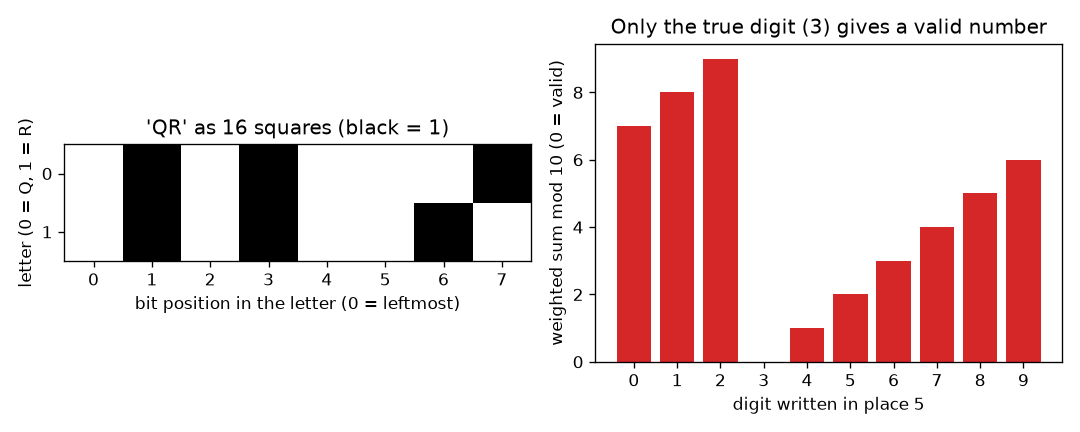
\includegraphics[width=0.85\linewidth]{figures/s01_squares_and_check.png}\\\small Left: the word QR as 16 squares. Right: only the true digit passes the check.\end{center}

\subsection*{E. Worked example}
Find the check digit of the 12 digits 400638133393 and say whether 4006381333931 is valid.
\begin{enumerate}[nosep]
\item Write the digits with weights 1, 3, 1, 3, ...: 4x1, 0x3, 0x1, 6x3, 3x1, 8x3, 1x1, 3x3, 3x1, 3x3, 9x1, 3x3.
\item Products: 4, 0, 0, 18, 3, 24, 1, 9, 3, 9, 9, 9.
\item Sum of the 12 products: S = 4 + 0 + 0 + 18 + 3 + 24 + 1 + 9 + 3 + 9 + 9 + 9 = 89.
\item The next multiple of 10 above 89 is 90, so the check digit is 90 - 89 = 1.
\item The full number is 4006381333931. Its 13 weighted terms add to 89 + 1x1 = 90, and 90 mod 10 = 0: valid.
\end{enumerate}
\textbf{Answer.} The check digit is 1, so 4006381333931 is valid (weighted sum 90).

\subsection*{F. Questions}
\begin{enumerate}[nosep]
\item \textbf{Conceptual.} Why can the check digit tell you that a number is wrong, but not which digit is wrong? What extra would you need to repair it?
\item \textbf{Numerical.} Find the check digit for the 12 digits 590123412345 and show the weighted sum.
\item \textbf{Graph and simulation interpretation.} In the graph of the weighted sum mod 10 against the digit written in place 6 (weight 3), how much does the remainder move when the digit goes up by 1? Why does exactly one digit give 0?
\item \textbf{Design and optimisation challenge.} Design: a library wants a check digit for 6-digit member numbers that catches EVERY swap of two neighbouring digits, which the EAN-13 rule does not (it misses digits that differ by 5). Propose a rule and state its cost.
\end{enumerate}

\section{Session 2: Parity bits and the Hamming(7,4) code}

\subsection*{A. Real-world problem}
A QR code on a bus ticket gets a scratch across a few squares, yet the gate still opens. The code must not only notice damage but repair it. What is the cheapest way to add extra bits so that ANY one flipped bit among them can be located and fixed? (General education only: this is a simplified model of the real, much stronger codes in QR standards.)

\subsection*{B. Concept and theory}
Work with bits and add modulo 2: 0+0=0, 0+1=1, 1+1=0 (the remainder after dividing by 2). The parity of some bits is their sum mod 2. Hamming(7,4) takes 4 data bits d1 d2 d3 d4 and appends 3 parity bits: p1 = d1+d2+d4, p2 = d1+d3+d4, p3 = d2+d3+d4. As a matrix: codeword = data x G (mod 2), where G is 4 by 7 and equals the 4 by 4 identity next to the parity rules P. The receiver multiplies the 7 received bits by the 3 by 7 parity-check matrix H = [P transposed \textbar{} identity] (mod 2). The 3-bit answer is the syndrome. It is 000 for a valid word. If bit k flips, the syndrome equals column k of H. The 7 columns are all different and non-zero, so the syndrome names the flipped bit, and we flip it back. The price is redundancy: 7 bits are sent for 4 bits of information, a code rate of 4/7 = 0.571. With r parity bits there are 2\textasciicircum{}r syndromes, which must name 'no error' and every one of the n = k + r positions, so 2\textasciicircum{}r \textgreater{}= k + r + 1. Bigger blocks waste fewer bits (rate rises) but protect only against one error per block. Two flipped bits in one block fool the decoder.

\begin{itemize}[nosep]
\item d1..d4: data bits (bit)
\item p1..p3: parity bits (bit)
\item G: generator matrix, 4 x 7 (no unit)
\item H: parity-check matrix, 3 x 7 (no unit)
\item s: syndrome, 3 bits (bit)
\item k, r, n: data bits, parity bits, block length n = k + r (bit)
\item R: code rate k / n (no unit)
\end{itemize}

\begin{equation*}
\mathbf c=\mathbf d\,G \pmod 2,\qquad G=\begin{pmatrix}I_4 & P\end{pmatrix},\quad H=\begin{pmatrix}P^{\mathsf T} & I_3\end{pmatrix}
\end{equation*}

\begin{equation*}
\mathbf s=H\,\mathbf r^{\mathsf T}\pmod 2;\quad \mathbf s=\mathbf 0\ \text{valid},\quad \mathbf s=\text{column }k\text{ of }H\ \Rightarrow\ \text{bit }k\text{ flipped}
\end{equation*}

\begin{equation*}
2^r\ \ge\ k+r+1,\qquad R=\frac{k}{k+r}
\end{equation*}

\begin{center}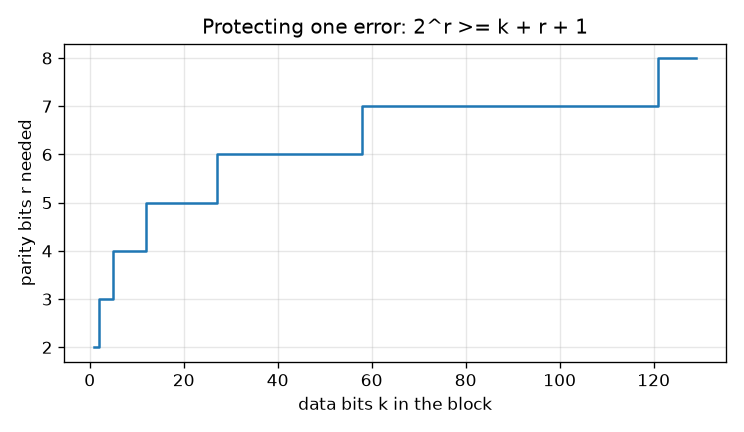
\includegraphics[width=0.85\linewidth]{figures/s02_parity_bits_needed.png}\\\small Parity bits needed against block size, from 2\textasciicircum{}r \textgreater{}= k + r + 1.\end{center}

\subsection*{E. Worked example}
Encode the data 1011, flip the third bit, and use the syndrome to find and fix it.
\begin{enumerate}[nosep]
\item Parity bits (mod 2): p1 = d1+d2+d4 = 1+0+1 = 2 -\textgreater{} 0; p2 = d1+d3+d4 = 1+1+1 = 3 -\textgreater{} 1; p3 = d2+d3+d4 = 0+1+1 = 2 -\textgreater{} 0.
\item Codeword: 1011 followed by 010, that is 1011010.
\item Flip bit 3: the receiver gets 1001010.
\item Syndrome, row 1 of H is 1101100: 1+0+0+1+0+0+0 = 2 -\textgreater{} 0. Row 2 is 1011010: 1+0+0+1+0+1+0 = 3 -\textgreater{} 1. Row 3 is 0111001: 0+0+0+1+0+0+0 = 1.
\item The syndrome 011 equals column 3 of H, so bit 3 is wrong. Flip it back: 1011010. The data are 1011 again.
\end{enumerate}
\textbf{Answer.} Codeword 1011010; received 1001010 has syndrome 011, which points at bit 3; the repaired data are 1011.

\subsection*{F. Questions}
\begin{enumerate}[nosep]
\item \textbf{Conceptual.} Why can a single parity bit detect one flipped bit but not repair it, while three overlapping parity checks can repair it?
\item \textbf{Numerical.} You receive 0100110 (Hamming(7,4) as in the lesson). Find the syndrome, the flipped bit and the data.
\item \textbf{Graph and simulation interpretation.} From the rate graph, what are the rates for r = 3, 4 and 5, and why does the rate rise with r? What do we lose?
\item \textbf{Design and optimisation challenge.} Design: you must protect 100 data bits, one error per block. Compare (a) one big block with (b) 25 separate Hamming(7,4) blocks, in parity bits, code rate and robustness.
\end{enumerate}

\section{Session 3: A toy matrix code, damaged and repaired}

\subsection*{A. Real-world problem}
A QR code on a parcel is scuffed, rained on and half covered by a sticker, yet it scans. How much damage can a code take before it fails, and how should its data be laid out so that a scratch does not kill it? We answer with a toy code you can fully understand. IMPORTANT: this toy code is NOT the QR standard. Real QR codes use Reed-Solomon codes over the finite field GF(256), with four error-correction levels L, M, Q and H that can restore roughly 7, 15, 25 and 30 percent of the codewords (well-known approximate figures), plus masking, alignment and timing patterns. We borrow only the ideas. (Simplified educational model, not a validated design tool.)

\subsection*{B. Concept and theory}
The message is 4 letters plus a check byte (the sum of the letters mod 256): 40 bits, 10 nibbles of 4 bits. Each nibble becomes a Hamming(7,4) codeword, so 70 bits go into a 12 by 12 grid whose three corners hold 3 by 3 finder patterns. Damage model: every data square flips independently with probability q (random noise), or a run of neighbouring squares flips (a burst). A block survives if it has at most one flipped bit out of 7: P\_block = (1-q)\textasciicircum{}7 + 7 q (1-q)\textasciicircum{}6 (no flips, or exactly one of the 7). The 10 blocks are independent, so the whole message survives with probability P\_block\textasciicircum{}10. A hard limit follows: if more than 10 of the 70 code squares are wrong, at least one block has two or more flips (pigeonhole), and decoding must fail. A repetition code that sends each bit n times (n odd) and takes a majority vote corrects up to (n-1)/2 flips per bit; with n = 3 it needs 120 squares for the 40 bits instead of 70. Interleaving: write the codewords as rows and send the columns, so that neighbouring squares belong to different codewords. With a group of g codewords, a burst of up to g neighbouring squares hits each codeword at most once, and Hamming repairs all of it.

\begin{itemize}[nosep]
\item q: probability that a data square is flipped (damage fraction) (no unit (0 to 1))
\item P\_block: probability a 7-bit block has at most 1 flip (no unit)
\item P\_msg: probability the whole message is read (no unit)
\item n: copies per bit in a repetition code (no unit)
\item g: interleave group (codewords written together) (codewords)
\item L: burst length (squares)
\end{itemize}

\begin{equation*}
P_{\text{block}}=(1-q)^7+7q(1-q)^6,\qquad P_{\text{msg}}=P_{\text{block}}^{\,10}
\end{equation*}

\begin{equation*}
P_{\text{rep}}=\left[\sum_{j=0}^{t}\binom{n}{j}q^j(1-q)^{n-j}\right]^{40},\quad t=\frac{n-1}{2}
\end{equation*}

\begin{equation*}
P_{\text{none}}=(1-q)^{40}
\end{equation*}

\begin{center}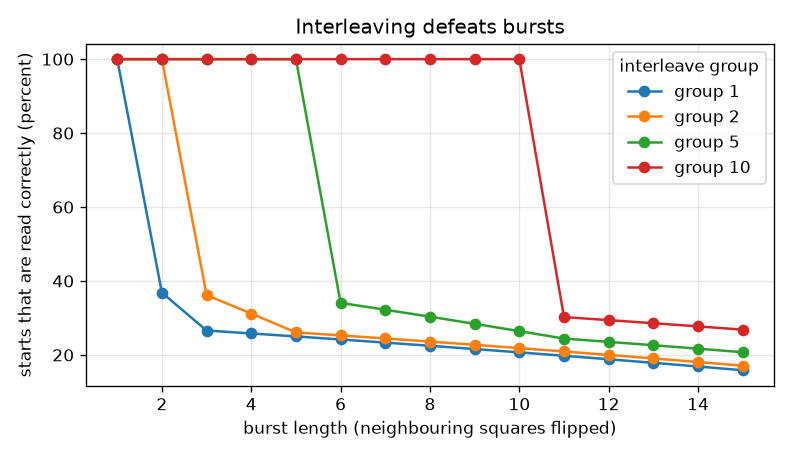
\includegraphics[width=0.85\linewidth]{figures/s03_burst_interleaving.png}\\\small Share of burst positions read correctly against burst length, for interleave groups 1, 2, 5 and 10.\end{center}

\subsection*{E. Worked example}
At q = 5 percent random damage, what is the probability that the toy code is read correctly? Compare with a simulation.
\begin{enumerate}[nosep]
\item No flips in a block: (0.95)\textasciicircum{}7 = 0.6983.
\item Exactly one flip in a block: 7 x 0.05 x (0.95)\textasciicircum{}6 = 0.35 x 0.7351 = 0.2573.
\item P\_block = 0.6983 + 0.2573 = 0.9556.
\item All 10 blocks must survive: P\_msg = 0.9556\textasciicircum{}10 = 0.635.
\item A simulation of the whole pipeline (build, damage, decode) with thousands of trials gives about 0.63 to 0.64, matching the formula.
\end{enumerate}
\textbf{Answer.} About 0.635: the toy code is read correctly in roughly 63 or 64 of 100 attempts at 5 percent random damage.

\subsection*{F. Questions}
\begin{enumerate}[nosep]
\item \textbf{Conceptual.} Why does writing the codewords as rows and sending the columns (interleaving) help against a scratch, even though it adds no new bits?
\item \textbf{Numerical.} For q = 2 percent, find P\_block and P\_msg for the toy code, and say how many of 100 parcels you expect to read.
\item \textbf{Graph and simulation interpretation.} In the success-versus-damage graph, at about which damage do the Hamming and the no-protection curves differ most, and what does the dashed line at 15.7 percent mean?
\item \textbf{Design and optimisation challenge.} Design: a label gets bursts of up to 7 squares. You may choose the interleave group 1, 2, 5 or 10. Which do you pick, and what is the price of choosing the largest group when random noise is also present?
\end{enumerate}

\section{Real-world mini-project}
\textbf{Choose the interleaving for a scratched parcel label.} A courier prints the toy code on parcels, and rollers scratch it with bursts of up to 7 neighbouring squares (in reading order). Session 3 lets you pick an interleave group of 1, 2, 5 or 10 codewords. Find the smallest group for which every burst of 1 to 7 squares, at every possible start position, is still read correctly.

\section{The path ahead}
\begin{enumerate}[nosep]
\item \textbf{Session 4: Survive a coffee-stain blob.} A 2D interleaving layout for the toy code and a test harness for square blobs.
\item \textbf{Session 5: Know when it failed.} A decoder that marks unreliable blocks instead of guessing, plus a stronger checksum.
\item \textbf{Session 6: Find the code in any orientation.} A reader that finds the three finder patterns and rotates the grid to upright before decoding.
\item \textbf{Session 7: Symbols instead of bits: Reed-Solomon.} A small Reed-Solomon encoder and decoder over GF(16) or GF(256).
\item \textbf{Session 8: Read a photograph.} A reader that takes a tilted greyscale picture of a code and recovers the message.
\end{enumerate}

\section{Answers and hints}

\subsection*{Session 1}
\begin{enumerate}[nosep]
\item \textbf{Conceptual.} Hint: The check gives one number between 0 and 9. How many different mistakes give the same remainder? Solution: The check compresses all 13 digits into one remainder. A remainder that is not 0 says 'some place changed', but many different places and digits give the same remainder, so it cannot name one. To repair a mistake you need several overlapping checks whose answers, together, point at one place. That is what the parity checks of Session 2 do.
\item \textbf{Numerical.} Hint: Use weights 1, 3, 1, 3, ... from the left. The check digit brings the sum up to the next multiple of 10. Solution: Products: 5x1=5, 9x3=27, 0x1=0, 1x3=3, 2x1=2, 3x3=9, 4x1=4, 1x3=3, 2x1=2, 3x3=9, 4x1=4, 5x3=15. Sum: 83. Next multiple of 10: 90, so the check digit is 7 and the number is 5901234123457. Sanity check: 83 + 7 = 90, which ends in 0.
\item \textbf{Graph and simulation interpretation.} Hint: Each step of 1 in the digit changes S by the weight of the place. Place 5 has weight 1 and its graph rises by 1 per step. Solution: With weight 3 the remainder jumps by 3 (mod 10) at each step: for the example number 4006381333931 the remainders for the digits 0 to 9 in place 6 are 6, 9, 2, 5, 8, 1, 4, 7, 0, 3. Because 3 and 10 share no factor, the ten digits give ten different remainders, so exactly one of them gives 0. The same holds for weight 1.
\item \textbf{Design and optimisation challenge.} Hint: Try weights that differ by something sharing no factor with the modulus, and think about which modulus works. Solution: Use a weighted sum modulo 11 with weights 7, 6, 5, 4, 3, 2 and choose the check value so that the total is a multiple of 11 (ISBN-10 works in a similar way). A swap of neighbours a, b changes the sum by (weight difference = 1) times (a minus b), and a - b is between -9 and 9 and non-zero, so it is never a multiple of 11: every swap is caught, and so is every single wrong digit. Cost: the check value can be 10, which needs an extra symbol (ISBN-10 writes X), so the numbers are no longer pure digits. Trade-off: stronger protection against swaps versus a more awkward format.
\end{enumerate}

\subsection*{Session 2}
\begin{enumerate}[nosep]
\item \textbf{Conceptual.} Hint: How many different answers can one parity bit give? How many can three give? Solution: One parity bit has two possible answers: 'fine' or 'wrong', so it cannot say where. Three overlapping checks give 3 bits, that is 8 possible syndromes: one for 'no error' and seven for 'bit k is wrong', k = 1 to 7. The checks overlap so that each bit is covered by a different pattern of checks, which makes its syndrome unique.
\item \textbf{Numerical.} Hint: Rows of H: 1101100, 1011010, 0111001. Multiply each with the received word and add mod 2. Solution: Row 1: 0+1+0+0+1+0+0 = 2 -\textgreater{} 0. Row 2: 0+0+0+0+0+1+0 = 1. Row 3: 0+1+0+0+0+0+0 = 1. Syndrome 011 = column 3, so bit 3 is wrong. Flipping it gives 0110110, so the data are 0110. Check: p1 = 0+1+0 = 1, p2 = 0+1+0 = 1, p3 = 1+1+0 = 0 matches the parity part 110.
\item \textbf{Graph and simulation interpretation.} Hint: Read the points (7,4), (15,11), (31,26): rate is k / n. Solution: Rates 4/7 = 0.571, 11/15 = 0.733, 26/31 = 0.839. The number of parity bits grows only like log2 of the block length while the data grow about twice as fast per extra parity bit, so the share of parity shrinks. What we lose: a block of 31 bits still repairs only ONE flip, so the longer the block, the less protection per bit.
\item \textbf{Design and optimisation challenge.} Hint: Use 2\textasciicircum{}r \textgreater{}= k + r + 1 for (a). For (b) each 4-bit group needs 3 parity bits. Solution: (a) k = 100 needs r = 7 (2\textasciicircum{}7 = 128 \textgreater{}= 108, while 2\textasciicircum{}6 = 64 \textless{} 107), so 107 bits are sent, rate 100/107 = 0.935, but only one flipped bit anywhere can be repaired. (b) 25 x 3 = 75 parity bits, 175 bits sent, rate 0.571, but up to 25 flips can be repaired if each lands in a different block. Trade-off: (a) is cheap but fragile, (b) costs 68 more bits but is robust against spread-out damage; real systems pick a middle path.
\end{enumerate}

\subsection*{Session 3}
\begin{enumerate}[nosep]
\item \textbf{Conceptual.} Hint: Where do the 7 bits of one codeword sit on the grid with and without interleaving? Solution: Without it the 7 bits of a codeword are neighbours, so a scratch of 2 squares puts 2 flips into one block, and Hamming cannot repair that. With group 10 the bits of one codeword are 10 squares apart, so a scratch of up to 10 squares hits each codeword at most once. The total number of flips is the same, but they are spread over many blocks, each with at most one: repairable.
\item \textbf{Numerical.} Hint: P\_block = (1-q)\textasciicircum{}7 + 7q(1-q)\textasciicircum{}6, then raise to the power 10. Solution: (0.98)\textasciicircum{}7 = 0.8681 and 7 x 0.02 x (0.98)\textasciicircum{}6 = 0.14 x 0.8858 = 0.1240, so P\_block = 0.9921. P\_msg = 0.9921\textasciicircum{}10 = 0.924. About 92 of 100 parcels. Sanity check: the lesson table prints 0.9242 for q = 0.02.
\item \textbf{Graph and simulation interpretation.} Hint: Look where the gap between the curves is largest and recall that 11 of the 70 code squares is the pigeonhole limit. Solution: They differ most at small damage, around 2 to 4 percent, where Hamming still reads 92 to 84 percent of codes while the unprotected 40 squares read only 45 to 30 percent. The dashed line at 11 / 70 = 15.7 percent marks the hard limit: with more than 10 wrong code squares some block must have two flips, so success is impossible beyond it. In practice success already collapses below 5 percent, long before the limit, because random flips pile up in some blocks.
\item \textbf{Design and optimisation challenge.} Hint: Use the guaranteed burst length (the largest burst that is always repaired) for each group from the lesson. Solution: The guaranteed burst length equals the group (1, 2, 5, 10 measured), so only group 10 handles 7. The measured survival of bursts of 7 squares is 23, 24 and 32 percent for groups 1, 2 and 5 and 100 percent for group 10. The price: interleaving costs nothing in extra bits and does not change the random-noise success (about 92 percent at q = 2 percent for every group), but the decoder needs all 10 blocks in one pass and the layout is harder to read by hand. Trade-off: no capacity cost, only complexity.
\end{enumerate}

\section{How to join}
Read \texttt{CONTRIBUTING.md} in the repository, then pick an issue labelled \texttt{good first issue}. Repository: \url{https://github.com/KrunalPanchal1995/openqrcode}

\end{document}
